%
% ritzAufProblem.tex 
%
% 
%
% !TEX root = ../../buch.tex
% !TEX encoding = UTF-8
%



\section{Ritz Verfahren angewandt\label{antennen:ritzAnw}}


Wie in REF erwähnt konnten wir dank der Symmetrie das Problem nur auf eine Ecke abbilden. 
Diese Ecke setze man nun geschickt wie in der Abbildung \ref{antennen:koordSysBsp} zu sehen 
in ein Koordinatensystem, welches uns erlaubt das Problem genauer zu analysieren.

%TODO bild ist weit weg [htbp] ILLEGAL
\begin{figure}%[htbp]
	\centering
	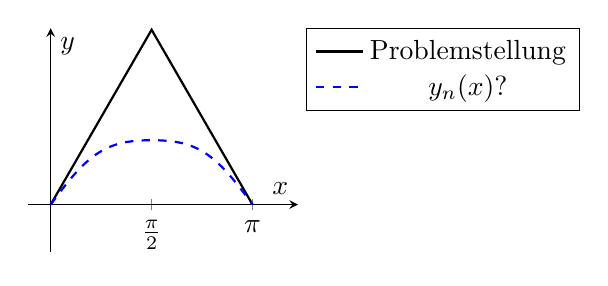
\begin{tikzpicture}
		\begin{axis}[
			scale=0.5,
			axis lines=middle,
			xlabel={$x$},
			ylabel={$y$},
			xtick={0, 1.5708, 3.14159},
			xticklabels={0, $\frac{\pi}{2}$, $\pi$},
			ytick=\empty,
			enlargelimits,
			clip=false,
			xmin=0, xmax=3.5,
			ymin=0, ymax=2,
			domain=0:pi, 
			samples=100,
			legend pos=outer north east,
			axis equal
			]
			% 3eck spitze
			\addplot[thick] coordinates {(0,0) (1.5708, pi*1.732/2) (3.14159, 0)};
			\addlegendentry{Problemstellung}
			
			\addplot[thick, blue, dashed, domain=0:3.14159, samples=100] {1.0882345*sin(deg(x))+0.0866761*sin(3*deg(x))};
			\addlegendentry{$y_n(x)?$}
		\end{axis}
	\end{tikzpicture}
	\caption{Problemstellung im Koordinatensystem}
	\label{antennen:koordSysBsp}
\end{figure}
Um die Effizienz $\eta$ zu optimieren, müssen wir mit der Approximationsfunktion
$y_n(x)$, wie in REF %~\ref{an} 
erwähnt, die quadrierte Fläche $A$ maximieren und die Länge $l$ minimieren.


\subsection{Nebenbedingungen von $y_n(x)$\label{antenennen:nebenbedRitz}}

Eine Nebenbedingung ist es, dass bei $y_n(0)$ und $y_n(\pi)$ die Funktion null sein muss.
Diese Nebenbedingung ist sehr wichtig für die Stetigkeit der finalen Form die wir optimieren.

Die Sinus-Fourier Reihe \eqref{antennen:unserRitz} hat eine weitere gute Eigenschaft, 
welche klar wird, wenn man in das gleiche Koordinatensystem wie bei der Abbildung \ref{antennen:koordSysBsp}
benützt und $y_n(x)$ mit beispielsweise den Koeffizienten $a_1=a_2=1$ plottet.

%TODO bild ist weit weg [htbp] ILLEGAL
\begin{figure}%[htbp]
	\centering
	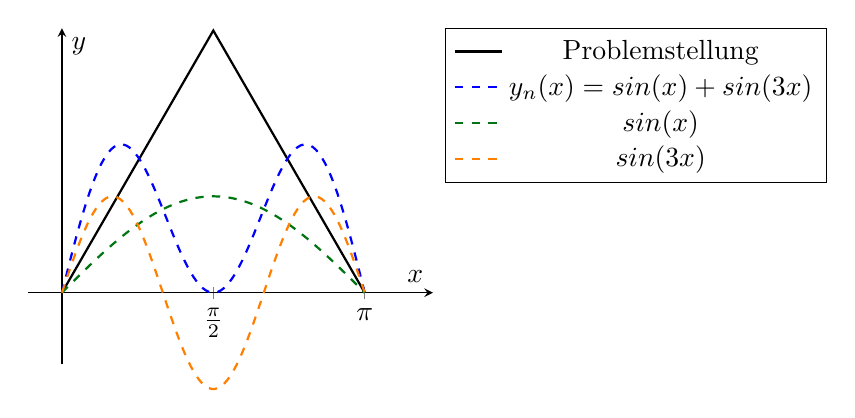
\begin{tikzpicture}
		\definecolor{clr1}{RGB}{0, 117, 18}
		\begin{axis}[
			scale=0.75,
			axis lines=middle,
			xlabel={$x$},
			ylabel={$y$},
			xtick={0, 1.5708, 3.14159},
			xticklabels={0, $\frac{\pi}{2}$, $\pi$},
			ytick=\empty,
			enlargelimits,
			clip=false,
			xmin=0, xmax=3.5,
			ymin=0, ymax=2,
			domain=0:pi, 
			samples=100,
			legend pos=outer north east,
			axis equal
			]
			% 3eck spitze
			\addplot[thick] coordinates {(0,0) (1.5708, pi*1.732/2) (3.14159, 0)};
			\addlegendentry{Problemstellung}
			
			\addplot[thick, blue, dashed, domain=0:3.14159, samples=100] {sin(deg(x))+sin(3*deg(x))};
			\addlegendentry{$y_n(x) = sin(x)+sin(3x)$}
			
			\addplot[thick, clr1, dashed, domain=0:3.14159, samples=100] {sin(deg(x))};
			\addlegendentry{$sin(x)$}
			
			\addplot[thick, orange, dashed, domain=0:3.14159, samples=100] {sin(3*deg(x))};
			\addlegendentry{$sin(3x)$}
		\end{axis}
	\end{tikzpicture}
	\caption{Nebenbedingungen im Koordinatensystem}
	\label{antennen:nebenbedGrafik}
\end{figure}

In der Abbildung \ref{antennen:nebenbedGrafik} ist zu sehen, dass dank der Punktsymmetrie 
der ungeraden Sinus-Funktionen, die Nebenbedingungen
\begin{equation}
	\begin{aligned}
		y_n(0)
		&=
		0
		\\
		y_n(\pi)
		&=
		0
	\end{aligned}
\label{antennen:nebenbed3eck}
\end{equation}
\em immer \em als \em erfüllt \em zu betrachten sind. Im weiteren Verlauf werden diese 
Nebenbedingungen somit nicht mehr beachtet.

\subsection{Die Lagrangefunktion \label{antennen:lagrangeFunktionen}}

%Die beste Fläche ist auch gerade die beste Fläche im quadrat \qed

Abstrahieren wir das Problem nun ein bisschen. Anstelle der Fläche $A$, reden wir nun von 
der Funktion $f$ und Länge $l$ wird zur Nebenbedingung $n$. 

An dieser Stelle sind unsere Koeffizienten $a_k$ konkret zu bestimmen. 
Somit sind die neu erwähnten Funktionen 

\begin{equation}
\begin{aligned}
	A
	\rightarrow
	f(a_1,\ldots,a_k)
	\rightarrow
	f(a_1,a_2)
	&=
	\int\limits_{0}^{\pi} y_n(x,a_1,a_2)\, dx
	\\
	l
	\rightarrow
	n(a_1,\ldots,a_k)
	\rightarrow
	n(a_1,a_2)
	&=
	\int\limits_{0}^{\pi} \sqrt{\frac{d}{d x} y_n\left(x, a_1, a_2\right)+1}\, dx
\end{aligned}
\label{antennen:lagrangeNamen}
\end{equation}


auch in deren Abhängigkeit bei \eqref{antennen:lagrangeNamen} zu sehen. 

Die Fläche unter der Kurve ergibt sich aus dem Integral der Funktion, 
während die Länge, also der obere Rand der Funktion, durch die in Kapitel REF  %\ref{label} 
erläuterte Formel berechnet wird. 

Die Nebenbedingung $n$ setzen wir nun gleich einer Konstanten Länge $\ell$
\begin{equation}
n(a_1, a_2)
=
\ell
\label{antennen:constNebenbed}
\end{equation}

und wie jede gute Nebenbedingung setzen wir diese noch gleich null

\begin{equation}
\begin{aligned}
	n(a_1, a_2) - \ell
	&=
	0
	\\
	n(a_1, a_2, \ell)
	&=
	0
\label{antennen:fertigeNebenbed}
\end{aligned}
\end{equation}

Nun kann man die Lagrangefunktion
\begin{equation}
L(x,a_1,a_2,\lambda)
= 
f(a_1,a_2)+\lambda \: n(a_1,a_2, \ell)
\end{equation}

definieren. Dazu wird die Funktion $f$ mit der Lagrange-Nebenbedingung $\lambda \: n$ addiert.
Mehr zu der Lagrangefunktion findet man unter dem Kapitel REF %\ref{label}

\subsection{Lagrange Gleichungssystem\label{antennen:lagrangeGLsys}}

Nun möchte man die Lagrangefunktion $L$ ableiten und 0 setzen. Nur heisst das in
diesem Kontext

% TODO GLsys bisschen spacen
\begin{equation}
	\nabla L = \vec{0} 
	\left\{ 
	\begin{aligned}
		\frac{\partial L}{\partial a_1} = 0 \\
		\frac{\partial L}{\partial a_2} = 0 \\
		\frac{\partial L}{\partial \lambda} = 0
	\end{aligned}
	\right.
	\label{antennen:lagrangeGrad}
\end{equation}

den Gradienten berechnen und dem Nullvektor gleichsetzen. Dabei entsteht hier ein 
$n+1$ dimensionales Gleichungssystem \eqref{antennen:lagrangeGrad}

An dieser Stelle soll es einem bewusst werden, was dieses Kapitel von anderen 
unterscheidet. Dank dem Verfahren nach Ritz konnten wir ein unendlich dimensionales
Problem, in ein endlich dimensionales verwandeln. 
Konkret heisst es, dass wir keine Differentialgleichung lösen müssen, sondern, 
das Gleichungssystem, welches wir bei \eqref{antennen:lagrangeGrad} erhalten haben.

Das Gleichungssystem \eqref{antennen:lagrangeGrad}, in diesem Fall mit 
2 Koeffizienten kann man dann als
\begin{equation}
	\begin{aligned}
		\int_0^\pi \sin (x) dx
		&=
		-\lambda \int_0^\pi \frac{\left(a_1 \cos (x)+3 a_2 \cos (3 x)\right) 
			\cos (x)}{\sqrt{\left(a_1 \cos (x)+3 a_2 \cos (3 x)\right)^2+1}} \, dx \\
		\int_0^\pi \sin (3 x) dx
		&=
		-\lambda \int_0^\pi \frac{3\left(a_1 \cos (x)+3 a_2 \cos (3 x)\right) 
			\cos (3 x)}{\sqrt{\left(a_1 \cos (x)+3 a_2 \cos (3 x)\right)^2+1}} \, dx \\
		\ell
		&=
		\int_0^\pi \sqrt{\left(a_1 \cos (x)+3 a_2 \cos (3 x)\right)^2+1} \, dx
	\end{aligned}
	\label{antennen:lagrangeGradKonkret}
\end{equation}
ausschreiben. 

\subsection{Das Gleichungssystem Lösen\label{antennen:glSysSolve}}

Ein gutes Verfahren, welches sich zur Lösung des Gleichungssystems 
\eqref{antennen:lagrangeGradKonkret}, anbietet, ist das Gradientenabstiegsverfahren.

Dieses iterative Verfahren eignet sich hervorragend zur Minimierung 
einer Funktion, indem man schrittweise in Richtung des steilsten Abstiegs,
also dem Gradienten aus der Gleichung \eqref{antennen:lagrangeGrad},
fortschreitet. 

% TODO nicht gute position, [htbp] illegal
\begin{figure}%[htbp]
	\centering
	\begin{tikzpicture}
		\begin{axis}[
			width=10cm,
			height=8cm,
			view={110}{40},
			grid=major,
			xlabel={$x$},
			ylabel={$y$},
			zlabel={$f(x,y)$},
			zmin=-1,
			zmax=5,
			domain=-1.5:1.25,
			y domain=-1.5:1.5,
			colormap={invertedcool}{color(0cm)=(magenta); color(0.5cm)=(cyan)},
			]
			\addplot3[
			mesh,
			shader=interp,
			samples=31,
			domain=-1.5:1.25,
			y domain=-1.5:1.5
			] {x^2 + y^2};
			
			\addplot3[
			thick,
			darkgreen,
			mark=*,
			mark options={solid},
			-stealth,
			line join=bevel,
			point meta=explicit symbolic,
			nodes near coords={
				\ifdim\coordindex pt=0pt Start\fi
				\ifdim\coordindex pt=7pt Ende\fi
			},
			every node near coord/.append style={anchor=south west, color=darkgreen}
			] coordinates {
				(-0.5, -1, 1.25)   
				(-0.429, -0.857, 0.918)
				(-0.357, -0.714, 0.638)
				(-0.286, -0.571, 0.408)
				(-0.214, -0.429, 0.230)
				(-0.143, -0.286, 0.102)
				(-0.071, -0.143, 0.026)
				(0, 0, 0)      
			};
		\end{axis}
	\end{tikzpicture}
	\caption{Gradientenverfahren auf $f(x,y)=x^2+y^2$}
	\label{antennen:gradverfahrenBSP}
\end{figure}

Ein Beispiel dafür wie das Verfahren aussehen kann, sieht man bei der 
Abbildung \ref{antennen:gradverfahrenBSP}. Man nimmt irgendeinen Startpunkt
und geht Schritt für Schritt in Richtung des $-\nabla$. Mit der Funktion
$f(x,y)=x^2+y^2$ ist dieses Verfahren recht einfach zu implementieren und ausführen.

Dieses Verfahren kommt jedoch auch mit einigen Tücken. Wenn die Funktion sehr komplex ist
und man die Schrittgrösse und Toleranz ungeschickt wählt, ist die Gefahr gross, dass man 
bei \em lokalen \em minimas Stecken bleibt, obwohl ein \em globales \em gesucht ist.

Da wir in unserer Arbeit ohnehin die Python-Bibliothek \texttt{SymPy} verwendet haben, 
um symbolische Berechnungen durchzuführen und automatisch $n$ Koeffizienten zu berechnen, 
konnten wir das Gleichungssystem \eqref{antennen:lagrangeGradKonkret} mithilfe der Funktion 
\texttt{nsolve()} lösen.

%TODO code im github?

Eventuell findet man den Code auf github?

\subsection{Auswertung der Lösung\label{antennen:auswertung}}

% TODO nicht gute position, [htbp] illegal
\begin{figure}%[htbp]
	\centering
	
	\definecolor{color1}{rgb}{1.0, 0.0, 1.0}
	\definecolor{color2}{rgb}{0.75, 0.0, 1.0}
	\definecolor{color3}{rgb}{0.5, 0.0, 1.0}
	\definecolor{color4}{rgb}{0.25, 0.0, 1.0}
	
	% 2 koeff
	\begin{subfigure}
		\centering
		\begin{tikzpicture}
			\begin{axis}[
				title={$n=2$ Koeffizienten},
				domain=0:pi,
				samples=100,
				ymin=0, ymax=3.5,
				xmin=0, xmax=3.5,
				axis lines=middle,
				xlabel={$x$},
				ylabel={$y$},
				xtick={0, 1.5708, 3.14159},
				xticklabels={0, $\frac{\pi}{2}$, $\pi$},
				ytick={0, 1, 2, 3},
				width=6cm, height=4cm
				]
				\addplot[thick, color1] {1.08823455130519*sin(deg(x)) + 0.0866761835928106*sin(3*deg(x))};
				\addplot[thick, color2] {1.81055138481242*sin(deg(x)) + 0.195685048731416*sin(3*deg(x))};
				\addplot[thick, color3] {2.46066609594305*sin(deg(x)) + 0.301243389027199*sin(3*deg(x))};
				\addplot[thick, color4] {3.08456094286871*sin(deg(x)) + 0.402479943701422*sin(3*deg(x))};
			\end{axis}
		\end{tikzpicture}
	\end{subfigure}%
	\hfill
	% 3 koeff
	\begin{subfigure}
		\centering
		\begin{tikzpicture}
			\begin{axis}[
				title={$n=3$ Koeffizienten},
				domain=0:pi,
				samples=100,
				ymin=0, ymax=3.5,
				xmin=0, xmax=3.5,
				axis lines=middle,
				xlabel={$x$},
				ylabel={$y$},
				xtick={0, 1.5708, 3.14159},
				xticklabels={0, $\frac{\pi}{2}$, $\pi$},
				ytick={0, 1, 2, 3},
				width=6cm, height=4cm
				]
				\addplot[thick, color1] {1.14063451060611*sin(deg(x)) + 0.108169939153489*sin(3*deg(x)) + 0.0268323654703764*sin(5*deg(x))};
				\addplot[thick, color2] {1.85437292911293*sin(deg(x)) + 0.253791821832382*sin(3*deg(x)) + 0.0683318364481152*sin(5*deg(x))};
				\addplot[thick, color3] {2.50955540772763*sin(deg(x)) + 0.402071210261300*sin(3*deg(x)) + 0.110183839692472*sin(5*deg(x))};
				\addplot[thick, color4] {3.14502916280716*sin(deg(x)) + 0.548044536721918*sin(3*deg(x)) + 0.150139877796318*sin(5*deg(x))};
			\end{axis}
		\end{tikzpicture}
	\end{subfigure}
	
	\vspace{0.5cm} 
	
	% 4l koeff
	\begin{subfigure}
		\centering
		\begin{tikzpicture}
			\begin{axis}[
				title={$n=4$ Koeffizienten},
				domain=0:pi,
				samples=100,
				ymin=0, ymax=3.5,
				xmin=0, xmax=3.5,
				axis lines=middle,
				xlabel={$x$},
				ylabel={$y$},
				xtick={0, 1.5708, 3.14159},
				xticklabels={0, $\frac{\pi}{2}$, $\pi$},
				ytick={0, 1, 2, 3},
				width=6cm, height=4cm
				]
				\addplot[thick, color1] {1.08336686654360*sin(deg(x)) + 0.102013525169225*sin(3*deg(x)) + 0.0292728737553532*sin(5*deg(x)) + 0.0100642932737197*sin(7*deg(x))};
				\addplot[thick, color2] {1.80275228117654*sin(deg(x)) + 0.262223597024550*sin(3*deg(x)) + 0.0898544624243682*sin(5*deg(x)) + 0.0312039886658123*sin(7*deg(x))};
				\addplot[thick, color3] {2.46107632379109*sin(deg(x)) + 0.430953350464770*sin(3*deg(x)) + 0.156100515783400*sin(5*deg(x)) + 0.0535838810399717*sin(7*deg(x))};
				\addplot[thick, color4] {3.10156229609598*sin(deg(x)) + 0.599148439503026*sin(3*deg(x)) + 0.221465165912620*sin(5*deg(x)) + 0.0748051312645227*sin(7*deg(x))};
			\end{axis}
		\end{tikzpicture}
	\end{subfigure}%
	\hfill
	% 5 koeff
	\begin{subfigure}
		\centering
		\begin{tikzpicture}
			\begin{axis}[
				title={$n=5$ Koeffizienten},
				domain=0:pi,
				samples=100,
				ymin=0, ymax=3.5,
				xmin=0, xmax=3.5,
				axis lines=middle,
				xlabel={$x$},
				ylabel={$y$},
				xtick={0, 1.5708, 3.14159},
				xticklabels={0, $\frac{\pi}{2}$, $\pi$},
				ytick={0, 1, 2, 3},
				width=6cm, height=4cm
				]
				\addplot[thick, color1] {1.08242048596654*sin(deg(x)) + 0.103364847431102*sin(3*deg(x)) + 0.0311161489593337*sin(5*deg(x)) + 0.0125977513219976*sin(7*deg(x)) + 0.00512952717128434*sin(9*deg(x))};
				\addplot[thick, color2] {1.79915900016821*sin(deg(x)) + 0.271669937694202*sin(3*deg(x)) + 0.102270415943148*sin(5*deg(x)) + 0.0453106859569591*sin(7*deg(x)) + 0.0178553921145572*sin(9*deg(x))};
				\addplot[thick, color3] {2.45687381390258*sin(deg(x)) + 0.451721838817908*sin(3*deg(x)) + 0.183206206667679*sin(5*deg(x)) + 0.0827190790444953*sin(7*deg(x)) + 0.0317715747685065*sin(9*deg(x))};
				\addplot[thick, color4] {3.09881979748560*sin(deg(x)) + 0.632286666812462*sin(3*deg(x)) + 0.264348386834190*sin(5*deg(x)) + 0.119443731427762*sin(7*deg(x)) + 0.0448574142367621*sin(9*deg(x))};
			\end{axis}
		\end{tikzpicture}
	\end{subfigure}
	
	\caption{Verschiedene Längen $\ell$ für $y_n(x)$ mit verschieden vielen Koeffizienten}
	\label{antenenn:plotskoeff}
\end{figure}

% TODO Fehler, n koeff bis unendlich, flaeche kreis vs meine FUnkt
Es wurde nun schon sehr oft erwähnt, dass wir die Fläche maximieren 
und Länge minimieren. 

Die plots sehen so aus \ref{antenenn:plotskoeff} 

% TODO in packages hinzufügen
\usetikzlibrary{pgfplots.fillbetween}

% TODO nicht gute position, [htbp] illegal
\begin{figure}%[htbp]
	\centering
	\begin{tikzpicture}
		\begin{axis}[
			axis lines=middle,
			xlabel=$x$,
			ylabel=$y$,
			xmin=0, xmax=3.14159, 
			xtick={0, 1.5708, 3.14159}, 
			xticklabels={0, $\frac{\pi}{2}$, $\pi$},
			axis equal=true, 
			every axis plot/.append style={thick}
			]
			\addplot[
			domain=0:3.14159,
			samples=200,
			red
			] 
			{1.7956133389*sin(deg(x)) + 0.28393414605*sin(deg(3*x)) + 0.117828104002*sin(deg(5*x)) + 0.0625789829*sin(deg(7*x)) + 0.036466961219*sin(deg(9*x))};
			
			\addplot[name path=F, domain=0:3.14159, samples=200, blue]
			{sqrt(1.5708^2-(x-1.5708)^2)};
			
			\path[name path=axis] (axis cs:0,0) -- (axis cs:3.14159,0);
			
			\addplot [
			thick,
			color=blue,
			fill=blue, 
			fill opacity=0.5,
			pattern=north east lines,
			pattern color=blue
			]
			fill between[
			of=F and axis,
			soft clip={domain=0:3.14159},
			split, 
			];
		\end{axis}
	\end{tikzpicture}
	\caption{$y_n(x)$ mit 8 Koeffizienten verglichen mit Kreis}
	\label{antennen:vergleichKreis}
\end{figure}
Beispiel Vergleich \ref{antennen:vergleichKreis} oder \ref{antennen:vergleichKreis2} hübscher?

\begin{figure}%[htbp]
	\centering
	\begin{tikzpicture}
		\begin{axis}[
			axis lines=middle,
			xlabel=$x$,
			ylabel=$y$,
			xmin=0, xmax=3.14159, 
			xtick={0, 1.5708, 3.14159}, 
			xticklabels={0, $\frac{\pi}{2}$, $\pi$},
			axis equal=true, 
			every axis plot/.append style={thick}
			]
			\addplot[
			domain=0:3.14159,
			samples=200,
			red
			] 
			{1.7956133389*sin(deg(x)) + 0.28393414605*sin(deg(3*x)) + 0.117828104002*sin(deg(5*x)) + 0.0625789829*sin(deg(7*x)) + 0.036466961219*sin(deg(9*x))};
			
			\addplot[name path=F, domain=0:3.14159, samples=200, blue]
			{sqrt(1.5708^2-(x-1.5708)^2)};
			
			\path[name path=axis] (axis cs:0,0) -- (axis cs:3.14159,0);
			
			\addplot [
			thick,
			color=blue,
			fill=blue, 
			fill opacity=0.5,
			pattern=dots,
			pattern color=blue
			]
			fill between[
			of=F and axis,
			soft clip={domain=0:3.14159},
			split, 
			];
		\end{axis}
	\end{tikzpicture}
	\caption{$y_n(x)$ mit 8 Koeffizienten verglichen mit Kreis}
	\label{antennen:vergleichKreis2}
\end{figure}














